%!TEX root = ../main.tex

\section{Architecture}

\begin{figure}[t]
  \centering
  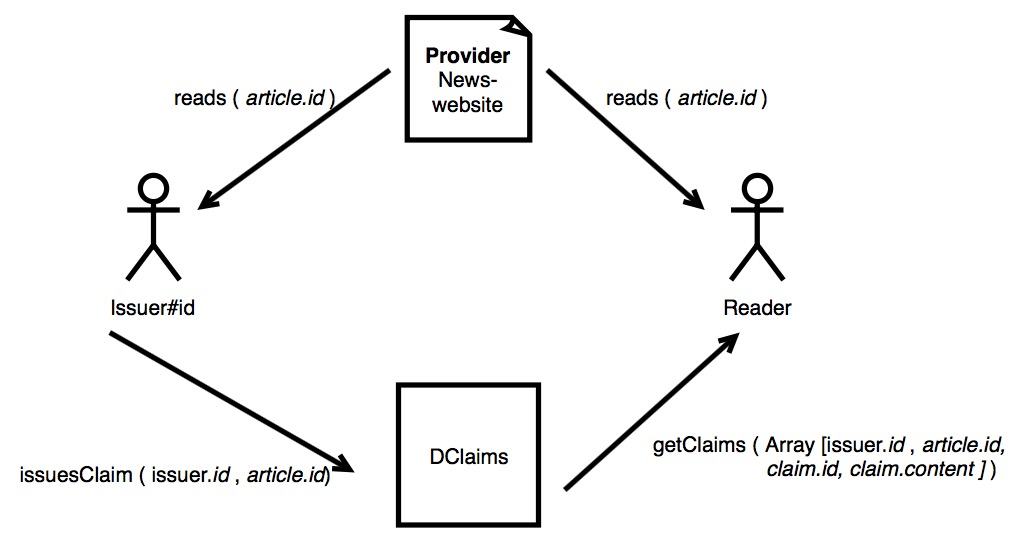
\includegraphics[width=0.8\columnwidth]{figures/arch.jpg}
% \vspace{5pt}
  \caption{DClaims architecture.}
% \vspace{-0.3cm}
  \label{fig:arch}
\end{figure}

Figure~\ref{fig:arch} presents the architecture of our system. 

\note{TODO:
- Need to  explain its core subcomponents: IPFS, Ethereum, and the browser plugin.
- Need to explain why using these components makes sense and discuss alternative approaches.
- Need to introduce two additional parties involved in the system workflow: publishers and curators.}

\subsection{Issuing a Claim flow}

\begin{figure}[t]
  \centering
  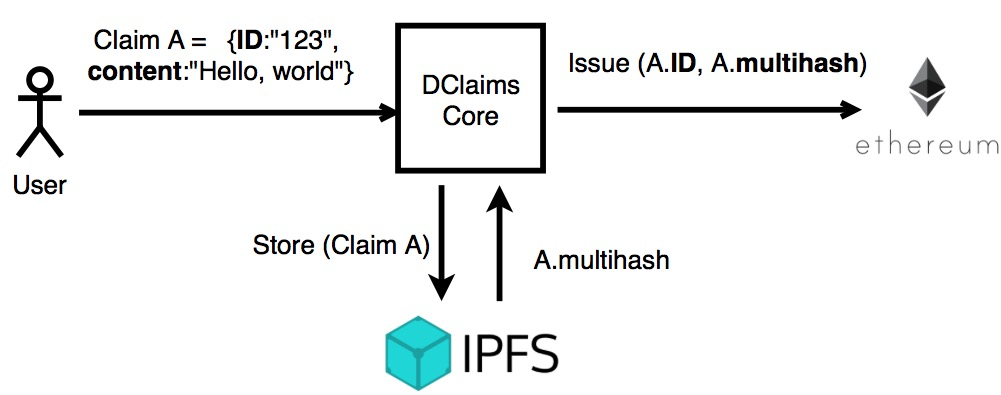
\includegraphics[width=0.8\columnwidth]{figures/arch2.jpg}
%  \vspace{5pt}
  \caption{DClaims issuance workflow.}
%  \vspace{-0.3cm}
  \label{fig:arch2}
\end{figure}

Figure \ref{fig:arch2} shows the issuing process.A user creates a Claim, A, with ID=123 and Content=“Hello, World”, DClaims adds that claim to IPFS, which returns the IPFS link (multihash), DClaims takes that ipfs-link and adds it to the Ethereum smart-contract, indexed by the ID. Meaning that for each ID there can be several claims. (note to self: change id to something better like index)

\subsubsection{Claims Discovery and Propagation}

Claims are stored on IPFS: Distributed file systems, Ensures the links don’t get broken.
An Ethereum smart-contract is used to keep track of the claims, Runs on a blockchain, Allows for the creation of smart-contracts (more about smart-contracts here), Turing complete

\subsection{Threat Model}

\note:{TODO: Here we need to properly characterize the attacker, what he can do, what he cannot do. Talk about what entities we trust.}

\subsection{Issuing and Verifying Claims}

\note:{TODO: Start by explaining the basic process for issuing and verifying claims involving IPFS and Ethereum. Then explain why IPFS and (in particular) Ethereum are important and necessary to make this work. Discuss other potential alternatives.}

\subsection{Costs and Incentives}

\note:{TODO: Here explain that by using Ethereum, costs will be involved. Talk about both the monetary costs of the issuing process and also the performance implications of relying on micro contracts. Then explain the solution based on publishers.}


\subsection{Claim Representation and Aggregation}

\note{TODO: Here explain the basic mechanism for representation of news, graphs between then, attaching more complex types of information, and dealing with a potentially large number of issuers and news. Talk about the curators as a solution for one of these problems.}

\subsection{Supporting Anonymous Sources}

\note{TODO: Talk about anonymous sources and how they can be supported. Talk also about the fact that it is going to be really difficult to revoke claims.}

\subsection{Resistance to censorship}

The application is executed locally, so news websites can not prevent users from running the extension on their website. The most they could do would be to change the name of the HTML classes, but we would quickly catch up.

Someone could still attack IPFS and Ethereum. \note{TODO: explain the thread model}

\subsection{Compatibility}

\note{TODO: Explain how easy it is to make work on any news-website.}

\subsection{Data Model}

Verifiable Claims are a data representation modal, proposed by the W3C Credentials Community Group \footnote{https://web.archive.org/web/20171013165205/https://www.w3.org/TR/verifiable-claims-data-model/} for describing achievements, qualities or other information.

An example would be a university digital diploma, singed by the university’s private key, that I can take to any employer and they can verify it. This diploma should continue to be verifiable even if the university ceases to exist.

Actions supported by Verifiable Claims:

\begin{itemize}
    \item Issue
    \item Share / retrieve
    \item Verify
    \item Revoke
\end{itemize}

What we want to do is to provide a platform that allows end users to have news items automatically reviewed by independent parties of their trust. News are understood as claims which are submitted to a review process. Figure~\ref{fig:model} shows how we envision it working. In our system there are three parties: providers, readers, and issuers. Providers are responsible for serving news content to the users on their browsers. Readers are nothing but the end users which visit providers' websites and browse through the news content. Issuers are responsible for reviewing certain news and issuing a certificate which will be associated to the news.

The idea is that the readers are able to check if some news items is reliable or fake depending on the endorsement produced by some issuer. Readers should be able to designate which issuers they trust so that by the time they visit a given website, each news item is classified according to the review generated by the issuer.

Note that it is not our goal to build a tool that can determine {\em per se} and automatically fake news. Our approach is instead to let readers establish trust relations with someone that they trust to provide them with reliable information. This can be, e.g., some original author, communities of experts, etc. Our system should allow issuers also to attach proofs of what they say is true. Put simply, we want to provide an instrument that can help news readers to mimic trust relations they have in the real world also in the virtual world.

\note{Organize all the stuff below}

\subsection{Publishers}

Entities that work as proxies to between issuers and the ethereum network.
Publishers receiver batch claims for a certain news article. When a publisher has receiver X (x being a treshold that can be defined by each publisher)
The single claims are batched into one larger claim, a batch, which is added to IPFS and issued in Ethereum as one transaction, which drops the price. Price of issuing one single claim = price of issuing a batch (which can have any number of single claims).
Publishers can then chose if they want to carry the cost of issuing to the issuers (100 claims from 100 different issuers, the ehthereum transaction price was 1USD, so each issuer would pay 0.01USD) or pay for the issuing themselves by implementing other mechanisms to generate revenue (display ads, have the issuers mine some cryptocurrency for them, mass adoption like review websites).

\paragraph{Misbehaved publishers: } Since publishers act as a proxy between issuers and the Ethereum smart-contract, in theory they could chose not to issue claims that they don’t like, effectively introducing censorship in the system. For that problem we have thought about two solutions, both based on the assumtption that everytime a issuer sends a claim to be issued by a publisher, the publisher replies with a receipt that a) acknowledges having received the claim (eg. returning the claim signed by the publisher) and b) has a prediction of when that claim will be issued (the block interval where that batch might be issued, eg. “your claim will be inserted in the batch with ID=X and should be inserted between blocks 1234567 and 1234590”).

\begin{enumerate}
    \item If the Issuers queries the blocks that he had on the receipt and verifies that the claim has not been inserted there, the Issuer could generate a new claim (issue it directly) where he proves (using the receipt) the publisher misbehaved. That claim could be issued in a “Bad-Publishers” smart-contract, which would warn the community not ti use that specific Publisher.
    \item A more dramatic, but possibly more effective approach would be to have publishers placing money in a smart-contract, as escrow. That smart-contract could receive “complaints” from issuers, which would contain the receipt sent by the publisher to that issuer. The smart-contract could then query the other smart contract (where the claim was supposed to be issued) and check if it had indeed been issued or not. If the smart-contract determined that the issue misbehaved, the value (or part of) the publisher had placed in escrow would be transfered to the complainant issuer. If batches are issued as a merkle tree, the merkle root would be the ipfs link and there is a great optimization that can be done here.
\end{enumerate}

\subsection{Curators}
Entities that take existing claims and generate new ones, based on the original ones.
Eg. "A Curator finds 100 claims about news article A. He would then issue a new claim saying something like ‘40% of claims classify this article as having a misleading title’ "
This would be useful for the end consumer, who could chose to subscribe to Curators rather than to individual issuers (Looking at a police report vs interviewing all the people involved in an event).

Curators could also create claims about articles that are similar to others.


\subsection{DClaims Web Extension}
The DClaims web extension creates a user interface on any news website that enables users to use the platform.
In its current form the DClaims web extension uses jQuery and Bootstrap for the user interface, Metamask and the Web3 library to communicate with Ethereum and the JS-IPFS-API to communicate with the IPFS daemon.
The DClaims web extension can be adapted to work on any news website with minimal configuration. As we will see in this section, DClaims starts by identifying the news website the user is on and then proceeds to learn if the user is in the website’s homepage or on a full article page.
News articles are identified by their URL and after having gathered the information about the news website and webpage (homepage or full article), DClaims generates IDs for each news article. One of two situations occur, either the user is visiting the homepage of the news website where multiple articles are displayed, or the user is in a full article page. In the first case, homepage, DClaims scrapes the entire webpage and looks for the URLs that each news article references and generates the article ID based on that URL. On the second case, full article page, the ID is generated based on the webpage’s URL (which will be the same that the article on the homepage was referencing). Let us now look into the behaviours in the homepage and full page.

\paragraph{Behaviour News Website’s Homepage}
In the homepage, DClaims enables user to view the claims made about each article displayed. The tasks it has to accomplish on the homepage are creating the visual elements to view claims, and claims count, made about each article. As stated before, the first step is to generate the ID for each article. After that, the HTML Document Object Model (DOM) elements are generated. DOM elements are connected to news articles via their ID, meaning a DOM element’s ID is the same as the ID of the article it serves.
The count of the number of claims is obtained by contacting the smart-contract, via Web3, and querying for that specific article.

\paragraph{Behaviour News Website’s Full Article Pages}
In a full article page, DClaims allows users to generate Claims about that article. As in the case of the homepage, DClaims starts by generating the article ID, followed by the creation of the HTML DOM elements, which in this case are a button to generate a claim and an pop up box with the claim fields to be filled by the user.

\subsection{DClaims Core component}

The DClaims core component handles communication with IPFS and Ethereum and it can run both on a Javascript (browser) or Node.js environment. It can be seen as the backend of the system, even though the concept of backed does not really apply here since we are dealing with a decentralized system.
 It connect to Ethereum using the Web3 object injected by Metamask, in the case of the browser extension, or it can connect directly to a Go-Ethereum (Geth) node, via the RPC.

DClaims core allows for the issuance and retrieval of claims, fetching the claims count for a given article ID and learning the identity of the current user.

\paragraph{Issuing a Claim}
In DClaims news articles are identified by an ID and to issue a claim DClaims receives the Claim object as well as the article id. The Claim object is stored on IPFS which returns the permanent and immutable link. After having the IPFS link, DClaims sends a transaction to the DClaims Ethereum smart-contract which calls the issue function with article ID and IPFS link as parameters. This results in a new entry on the smart-contract’s  articles claims hash list.
DClaims than returns the transaction ID in case the user wants to check the transaction confirmation status.

\paragraph{Getting a claim}
tbd

